%
% A header that lets you compile a chapter by itself, or inside a larger document.
% Adapted from http://stackoverflow.com/a/3655553/751077
% Use \inbpdocument and \outbpdocument in your individual files, in place of \begin{document} and \end{document}.
% In your main file, put in a \def \ismaindoc {} before including or importing anything.


\ifx\ismaindoc\undefined
    \newcommand{\inbpdocument}{
        \def \ismaindoc {}
        % Use this header if we are compiling by ourselves.
        \documentclass[a4paper,12pt,twoside]{report}
        
\usepackage{graphicx}
\usepackage{verbatim}
\usepackage{latexsym}
\usepackage{mathchars}
\usepackage{setspace}
\usepackage[left=2cm,right=2cm,top=2cm,bottom=3cm]{geometry}
\usepackage[inline]{enumitem}
\usepackage[utf8]{inputenc}
\usepackage{hyperref}
\usepackage{natbib}
\usepackage{authordate1-4}
\usepackage{appendix}
\usepackage[nottoc]{tocbibind} % add Bibliography to toc
\usepackage{caption}
\usepackage{subcaption}
\usepackage{booktabs}
\usepackage{longtable}
\usepackage{algorithm2e}
\usepackage{float}
\usepackage{amsmath}
% \restylefloat{table}

\hypersetup{linktoc=all}
% \usepackage{url}

\setcounter{secnumdepth}{4}
\setcounter{tocdepth}{4}


\setlength{\parskip}{\medskipamount}  % a little space before a \par
\setlength{\parindent}{0pt}	      % don't indent first lines of paragraphs

%UHEAD.STY  If this is included after \documentstyle{report}, it adds
% an underlined heading style to the LaTeX report style.
% \pagestyle{uheadings} will put underlined headings at the top
% of each page. The right page headings are the Chapter titles and
% the left page titles are supplied by \def\lefthead{text}.

% Ted Shapin, Dec. 17, 1986

\makeatletter
\def\chapapp2{Chapter}

% \def\appendix{\par
%  \setcounter{chapter}{0}
%  \setcounter{section}{0}
%  \def\chapapp2{Appendix}
%  \def\@chapapp{Appendix}
%  \def\thechapter{\Alph{chapter}}}

\def\ps@uheadings{\let\@mkboth\markboth
% modifications
\def\@oddhead{\protect\underline{\protect\makebox[\textwidth][l]
		{\sl\rightmark\hfill\rm\thepage}}}
\def\@oddfoot{}
\def\@evenfoot{}
\def\@evenhead{\protect\underline{\protect\makebox[\textwidth][l]
		{\rm\thepage\hfill\sl\leftmark}}}
% end of modifications
\def\chaptermark##1{\markboth {\ifnum \c@secnumdepth >\m@ne
 \chapapp2\ \thechapter. \ \fi ##1}{}}%
\def\sectionmark##1{\markright {\ifnum \c@secnumdepth >\z@
   \thesection. \ \fi ##1}}}
\makeatother



%%From: marcel@cs.caltech.edu (Marcel van der Goot)
%%Newsgroups: comp.text.tex
%%Subject: illegal modification of boxit.sty
%%Date: 28 Feb 92 01:10:02 GMT
%%Organization: California Institute of Technology (CS dept)
%%Nntp-Posting-Host: andromeda.cs.caltech.edu
%%
%%
%%Quite some time ago I posted a file boxit.sty; maybe it made it
%%to some archives, although I don't recall submitting it. It defines
%%	\begin{boxit}
%%	...
%%	\end{boxit}
%%to draw a box around `...', where the `...' can contain other
%%environments (e.g., a verbatim environment). Unfortunately, it had
%%a problem: it did not work if you used it in paragraph mode, i.e., it
%%only worked if there was an empty line in front of \begin{boxit}.
%%Luckily, that is easily corrected.
%%
%%HOWEVER, apparently someone noticed the problem, tried to correct it,
%%and then distributed this modified version. That would be fine with me,
%%except that:
%%1. There was no note in the file about this modification, it only has my
%%   name in it.
%%2. The modification is wrong: now it only works if there is *no* empty
%%   line in front of \begin{boxit}. In my opinion this bug is worse than
%%   the original one.
%%
%%In particular, the author of this modification tried to force an empty
%%line by inserting a `\\' in the definition of \Beginboxit. If you have
%%a version of boxit.sty with a `\\', please delete it. If you have my
%%old version of boxit.sty, please also delete it. Below is an improved
%%version.
%%
%%Thanks to Joe Armstrong for drawing my attention to the bug and to the
%%illegal version.
%%
%%                                          Marcel van der Goot
%% .---------------------------------------------------------------
%% | Blauw de viooltjes,                    marcel@cs.caltech.edu
%% |    Rood zijn de rozen;
%% | Een rijm kan gezet
%% |    Met plaksel en dozen.
%% |


% boxit.sty
% version: 27 Feb 1992
%
% Defines a boxit environment, which draws lines around its contents.
% Usage:
%   \begin{boxit}
%	... (text you want to be boxed, can contain other environments)
%   \end{boxit}
%
% The width of the box is the width of the contents.
% The boxit* environment behaves the same, except that the box will be
% at least as wide as a normal paragraph.
%
% The reason for writing it this way (rather than with the \boxit#1 macro
% from the TeXbook), is that now you can box verbatim text, as in
%   \begin{boxit}
%   \begin{verbatim}
%   this better come out in boxed verbatim mode ...
%   \end{verbatim}
%   \end{boxit}
%
%						Marcel van der Goot
%						marcel@cs.caltech.edu
%

\def\Beginboxit
   {\par
    \vbox\bgroup
	   \hrule
	   \hbox\bgroup
		  \vrule \kern1.2pt %
		  \vbox\bgroup\kern1.2pt
   }

\def\Endboxit{%
			      \kern1.2pt
		       \egroup
		  \kern1.2pt\vrule
		\egroup
	   \hrule
	 \egroup
   }	

\newenvironment{boxit}{\Beginboxit}{\Endboxit}
\newenvironment{boxit*}{\Beginboxit\hbox to\hsize{}}{\Endboxit}

\pagestyle{empty}

\setlength{\parskip}{2ex plus 0.5ex minus 0.2ex}
\setlength{\parindent}{0pt}

\makeatletter  %to avoid error messages generated by "\@". Makes Latex treat "@" like a letter

\linespread{0.66}
\def\submitdate#1{\gdef\@submitdate{#1}}
\def\supervisor#1{\gdef\@supervisor{Supervisor: #1}}

\def\maketitle{
  \begin{titlepage}{
    %\linespread{1.5}
    \Large Queen Mary, University of London \\
    %\linebreak
    Department of Electronic Engineering and Computer Science
    \rm
    \vskip 3in
    \Large \bf \@title \par
  }
  \vskip 0.3in
  \par
  {\Large \@author}
  \vskip 0.1in
  {\Large \@supervisor}

  \vskip 4in
  \par
  Submitted in part fulfilment of the requirements for the degree of
  \linebreak
  BSc Computer Science with Industrial Experience, \@submitdate
  \vfil
  \end{titlepage}
}

\def\titlepage{
  \newpage
  \centering
  \linespread{1}
  \normalsize
  \vbox to \vsize\bgroup\vbox to 9in\bgroup
}
\def\endtitlepage{
  \par
  \kern 0pt
  \egroup
  \vss
  \egroup
  \cleardoublepage
}

\def\abstract{
  \begin{center}{
    \large\bf Abstract}
  \end{center}
  \small
  %\def\baselinestretch{1.5}
  \linespread{1.5}
  \normalsize
}
\def\endabstract{
  \par
}

\newenvironment{acknowledgements}{
  \cleardoublepage
  \begin{center}{
    \large \bf Acknowledgements}
  \end{center}
  \small
  \linespread{1.5}
  \normalsize
}{\cleardoublepage}
\def\endacknowledgements{
  \par
}

\newenvironment{dedication}{
  \cleardoublepage
  \begin{center}{
    \large \bf Dedication}
  \end{center}
  \small
  \linespread{1.5}
  \normalsize
}{\cleardoublepage}
\def\enddedication{
  \par
}

\def\preface{
    \pagenumbering{roman}
    \pagestyle{plain}
    \doublespacing
}

\def\body{
    \cleardoublepage
    \pagestyle{uheadings}
    \singlespacing
    \tableofcontents
    \doublespacing
    \normalsize
    \pagestyle{plain}

    \cleardoublepage
    \pagestyle{uheadings}
    \listoftables
    \pagestyle{plain}

    \cleardoublepage
    \pagestyle{uheadings}
    \listoffigures
    \pagestyle{plain}

    \cleardoublepage
    \pagestyle{uheadings}
    \pagenumbering{arabic}
    % \doublespacing
}

\makeatother  %to avoid error messages generated by "\@". Makes Latex treat "@" like a letter


\newcommand{\ipc}{{\sf ipc}}

\newcommand{\Prob}{\bbbp}
\newcommand{\Real}{\bbbr}
\newcommand{\real}{\Real}
\newcommand{\Int}{\bbbz}
\newcommand{\Nat}{\bbbn}

\newcommand{\NN}{{\sf I\kern-0.14emN}}   % Natural numbers
\newcommand{\ZZ}{{\sf Z\kern-0.45emZ}}   % Integers
\newcommand{\QQQ}{{\sf C\kern-0.48emQ}}   % Rational numbers
\newcommand{\RR}{{\sf I\kern-0.14emR}}   % Real numbers
\newcommand{\KK}{{\cal K}}
\newcommand{\OO}{{\cal O}}
\newcommand{\AAA}{{\bf A}}
\newcommand{\HH}{{\bf H}}
\newcommand{\II}{{\bf I}}
\newcommand{\LL}{{\bf L}}
\newcommand{\PP}{{\bf P}}
\newcommand{\PPprime}{{\bf P'}}
\newcommand{\QQ}{{\bf Q}}
\newcommand{\UU}{{\bf U}}
\newcommand{\UUprime}{{\bf U'}}
\newcommand{\zzero}{{\bf 0}}
\newcommand{\ppi}{\mbox{\boldmath $\pi$}}
\newcommand{\aalph}{\mbox{\boldmath $\alpha$}}
\newcommand{\bb}{{\bf b}}
\newcommand{\ee}{{\bf e}}
\newcommand{\mmu}{\mbox{\boldmath $\mu$}}
\newcommand{\vv}{{\bf v}}
\newcommand{\xx}{{\bf x}}
\newcommand{\yy}{{\bf y}}
\newcommand{\zz}{{\bf z}}
\newcommand{\oomeg}{\mbox{\boldmath $\omega$}}
\newcommand{\res}{{\bf res}}
\newcommand{\cchi}{{\mbox{\raisebox{.4ex}{$\chi$}}}}
%\newcommand{\cchi}{{\cal X}}
%\newcommand{\cchi}{\mbox{\Large $\chi$}}

% Logical operators and symbols
\newcommand{\imply}{\Rightarrow}
\newcommand{\bimply}{\Leftrightarrow}
\newcommand{\union}{\cup}
\newcommand{\intersect}{\cap}
\newcommand{\boolor}{\vee}
\newcommand{\booland}{\wedge}
\newcommand{\boolimply}{\imply}
\newcommand{\boolbimply}{\bimply}
\newcommand{\boolnot}{\neg}
\newcommand{\boolsat}{\!\models}
\newcommand{\boolnsat}{\!\not\models}


\newcommand{\op}[1]{\mathrm{#1}}
\newcommand{\s}[1]{\ensuremath{\mathcal #1}}

% Properly styled differentiation and integration operators
\newcommand{\diff}[1]{\mathrm{\frac{d}{d\mathit{#1}}}}
\newcommand{\diffII}[1]{\mathrm{\frac{d^2}{d\mathit{#1}^2}}}
\newcommand{\intg}[4]{\int_{#3}^{#4} #1 \, \mathrm{d}#2}
\newcommand{\intgd}[4]{\int\!\!\!\!\int_{#4} #1 \, \mathrm{d}#2 \, \mathrm{d}#3}

% Large () brackets on different lines of an eqnarray environment
\newcommand{\Leftbrace}[1]{\left(\raisebox{0mm}[#1][#1]{}\right.}
\newcommand{\Rightbrace}[1]{\left.\raisebox{0mm}[#1][#1]{}\right)}

% Funky symobols for footnotes
\newcommand{\symbolfootnote}{\renewcommand{\thefootnote}{\fnsymbol{footnote}}}
% now add \symbolfootnote to the beginning of the document...

\newcommand{\normallinespacing}{\renewcommand{\baselinestretch}{1.5} \normalsize}
\newcommand{\mediumlinespacing}{\renewcommand{\baselinestretch}{1.2} \normalsize}
\newcommand{\narrowlinespacing}{\renewcommand{\baselinestretch}{1.0} \normalsize}
\newcommand{\bump}{\noalign{\vspace*{\doublerulesep}}}
\newcommand{\cell}{\multicolumn{1}{}{}}
\newcommand{\spann}{\mbox{span}}
\newcommand{\diagg}{\mbox{diag}}
\newcommand{\modd}{\mbox{mod}}
\newcommand{\minn}{\mbox{min}}
\newcommand{\andd}{\mbox{and}}
\newcommand{\forr}{\mbox{for}}
\newcommand{\EE}{\mbox{E}}

\newcommand{\deff}{\stackrel{\mathrm{def}}{=}}
\newcommand{\syncc}{~\stackrel{\textstyle \rhd\kern-0.57em\lhd}{\scriptstyle L}~}

\def\coop{\mbox{\large $\rhd\!\!\!\lhd$}}
\newcommand{\sync}[1]{\raisebox{-1.0ex}{$\;\stackrel{\coop}{\scriptscriptstyle
#1}\,$}}

\newtheorem{definition}{Definition}[chapter]
\newtheorem{theorem}{Theorem}[chapter]

\newcommand{\Sectionref}[1]{Section~\ref{#1}}
\newcommand{\Tableref}[1]{Table~\ref{#1}}
\newcommand{\Pageref}[1]{page~\pageref{#1}}

\newcommand{\Figref}[1]{Figure~\ref{#1}}
\newcommand{\fig}[3]{
 \begin{figure}[!ht]
 \begin{center}
 \scalebox{#3}{\includegraphics{figs/#1.ps}}
 \vspace{-0.1in}
 \caption[ ]{\label{#1} #2}
 \end{center}
 \end{figure}
}

\newcommand{\figtwo}[8]{
 \begin{figure}
 \parbox[b]{#4 \textwidth}{
 \begin{center}
 \scalebox{#3}{\includegraphics{figs/#1.ps}}
 \vspace{-0.1in}
 \caption{\label{#1}#2}
 \end{center}
 }
 \hfill
 \parbox[b]{#8 \textwidth}{
 \begin{center}
 \scalebox{#7}{\includegraphics{figs/#5.ps}}
 \vspace{-0.1in}
 \caption{\label{#5}#6}
 \end{center}
 }
 \end{figure}
}

        \normallinespacing
        \begin{document}
    }
    \newcommand{\outbpdocument}[1]{
      % Fake chapters so references aren't broken
        \label{cha:introduction}
        \label{cha:background}
        \label{cha:data-classification}
        \label{cha:topic-modelling}

        \bibliographystyle{authordate1}
        \bibliography{bibliography}
        \end{document}
    }
\else
    %If we're inside another document, no need to re-start the document.
    \ifx\inbpdocument\undefined
        \newcommand{\inbpdocument}{}
        \newcommand{\outbpdocument}[1]{}
    \fi
\fi

\inbpdocument

\chapter{Background Theory}

\label{ch:background}

\section{Introduction}
\label{sec:background-introduction}
% In this chapter, we explain some concepts and take a look at some background work related to this
% study. Firstly, we review some research in the use of the naive Bayes Classifier for text
% classification. Then we take a look at some background in topic modelling, specifically the Latent
% Dirichlet Allocation

Automatic Text Classification or Text Categorisation is a rapidly growing field in Machine Learning
and Natural Language Processing. This is mainly due to the amount of electronic data we currently
generate. The main task is to assign one or more classes to a given text document. Some applications
of text classification include \textit{Email Spam Detection} and \textit{Language Detection}. The
former involves trying to distinguish spam emails from legitimate ones while the latter involves the
identification of the language a document was written in.

However, this study makes use of classification techniques for data filtration which involves
removing irrelevant documents from a list of documents(similar to spam filtering) and topic
modelling (extracting topics from a list of documents) and sentiment analysis (predicting the
sentiment of the author of a document). This chapter explains a few background concepts and reviews
some relevant research previously done in this area.

\section{Na\"{i}ve Bayes Classifier}
\label{sec:bg-naive-bayes}
The Na\"{i}ve Bayes classifier is one of the simplest classifier that can be used and this is due to
the fact that it is based on simple Bayes Theorem. It is a probabilistic classifier which assumes
that all features of the documents are independent of each other. This means that if a document has
features $f1$ and $f2$ (could be length of document, occurrence of words e.t.c), the
existence of $f1$ has nothing to do with the existence of $f2$ and vice versa. This also means that
it makes assumptions that may or may not be correct, hence the ``Na\"{i}ve'' in its name.

Bayes theorem states that the probability of $A$ given $B$ is the probability of $B$ given $A$ times
the probability of $A$ divided by the probability of $B$. Mathematically, this is written as:
\begin{equation}
  p(A|B) = \frac{p(B|A)p(A)}{p(B)}
\end{equation}

Applying this logic to text classification, the probability that a document $d_i \in D$ belongs to a
class $c$ is denoted as:
\begin{equation}
  p(c|d_i) = \frac{p(d_i|c)p(c)}{p(d_i)}
\end{equation}

% TODO: Show the final equation for the naive bayes classifier
Although other techniques like Maximum Entropy, Random Forests or Support Vector Machines tend to
perform better, a naive Bayes classifier will require less memory and CPU cycles. Furthermore, it is
computationally less complex and simpler to implement. With regard to
performance,~\citet{huangLuLing2003} showed using multiple datasets from~\citet{blakeMerz1998} that
the naive Bayes classifier in many cases performs as good as other complex classifiers
and~\citet{zhang2004} goes further to explain why it performs well. Other studies have also found
Bayesian classifiers to be effective without being affected by its simple independence
assumption~\citep{langley1992analysis,manning2008}.

The Na\"{i}ve Bayes classifier has been used in many text classification problems but one of its
common applications which is relevant to tweet classification is email spam\footnote{irrelevant or
unsolicited messages. They are typically to large numbers of users} filtering. A spam
filter is a system that takes in text and decides whether or not it is
spam. \citet{androutsopoulos2000learning} addressed this issue using a naive Bayes classifier. They
trained the model using a predefined set of manually labelled messages. They were able to show that
the naive Bayes classifier was capable of classifying messages with impressive accuracy and precision
compared to the then common keyword based approach to classification. \citet{deshpande2007evaluation}
also carried out a similar research and the results were equally impressive and similar.

\section{Topic Modelling}
\label{sec:bg-topic-modelling}
Topic Modelling is a process by which abstract topics/themes are extracted from a collection of
documents. This process is usually carried out with the aid of topic models, a suite of algorithms
used for topic modelling. It has been applied in a variety of fields like Software Analysis
where~\citet{linstead2009software} used topic modelling to find topics embedded in code
and~\citet{gethers2010using} used topic modelling to capture coupling among
classes.~\citet{kireyev2009applications} applied topic models on disaster related data from Twitter
in an effort to determine what topics were discussed within the time span of a natural
disaster.~\citet{hospedales2009markov} introduced a new topic model that can be used to analyze
videos with complex and crowded scenes in other to discover regularities in the videos. A system
built on such model will be able to answer a question like ``What interesting events happened in the
last 5 hours''. Other fields include Audio Analysis~\citep{smaragdis2009topic}, Influence
modelling~\citep{gerrish2009modeling}, Finance~\citep{doyle2009financial}, Writer
Identification~\citep{bhardwaj2009writer} and many more.

There are a number of topic models but the two main ones are \textbf{\textit{Latent Semantic
Indexing}} (LSI) and \textbf{\textit{Latent Dirichlet Allocation}} (LDA) and we discuss them further
in the following sections.


\subsection{Latent Semantic Indexing}
\label{sub:bg-lsa}
Latent Semantic Indexing(LSI) \citep{hofmann1999probabilistic}, sometimes referred to as
\textit{Latent Semantic Analysis}, is an indexing technique that leverages matrix-algebra
computations\footnote{Specifically, it uses Singular Value Decomposition which is a factorization of
a complex matrix. See \url{http://en.wikipedia.org/wiki/Singular_value_decomposition}} to identify
any patterns in relationships between a collection of text documents. It works based on the
assumption that words used in the same context tend to have homogeneous meanings
\citep{deerwester1990indexing,dumais2004latent,landauer2006latent}. LSI, has been used mostly in
Information Retrieval and Search Engine Optimisation where it tries to figure out what words in a
web page are relevant to the web page even though they might not be used in that page. One of the
main drawbacks the LSI model suffers from is ambiguity.

Assuming we have two documents, one talking about Microsoft Office and the other talking about
actual physical office space. How can the model differentiate between the two? Unfortunately, it is
unable to differentiate between such topics and a significant step to solve this problem was made by
\citet{hofmann1999probabilistic} who presented the probabilistic LSI model. \citet{blei2003latent}
argues that while Hoffman's work is a very useful step towards using probabilistic models to model
text, it is incomplete.

\subsection{Latent Dirichlet Allocation}
\label{sec:bg-lda}

\begin{figure}[H]
\begin{center}
    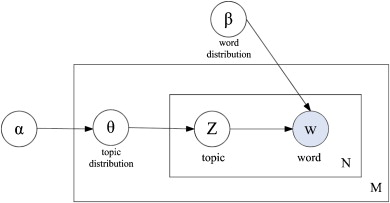
\includegraphics[scale=1.5]{Figures/lda}
\end{center}
\caption{A graphical model representation of LDA (Courtesy: \url{http://victorfang.wordpress.com/2012/03/11/latent-dirichlet-allocation})}
\label{fig:lda}
\end{figure}

Latent Dirichlet Allocation(LDA) is a generative\footnote{See
\url{http://en.wikipedia.org/wiki/Generative_model}} and probabilistic model that can be used to
automatically group words into topics and documents into a mixture of topics \citep{blei2003latent}.
It works based on the assumption that each document contains one or more topics. Words can also
exist in multiple topics as they actually do in natural language. In other to tackle the problem of
ambiguity LSI suffers from, LDA takes a combination of all topics that seem relevant
to a document in a corpora\footnote{Corpora is simply a large collection of documents} and compares
that document to the topics in an effort to determine which topic is closer to the document.
\Figref{fig:lda} shows a graphical model representation of Latent Dirichlet Allocation. The inner
boxes represents the choice of topics and words within a document while the outer box represents the
actual documents.

\citet{hoffman2010online} developed a variant of LDA called Online LDA which uses variational
Bayes as its posterior inference algorithm as opposed to Gibbs Sampling. It also allows the model to
be updated with more data after initial training. During initial training, the entire corpora is
observed/trained in batches rather than at once. \citet{asuncion2009smoothing} shows that although
this model uses constant memory and it converges quicker, it still requires a full pass through the
entire corpora. This makes it very slow when applied to large datasets.

An oversimplified version of the algorithm is:\\
\begin{algorithm}[H]
  \While{model is yet to converge} {%
    \KwData{$B =$ randomly selected mini-batch of documents\;}
    \For{$b\in B$}{%
      Estimate approximate posterior over what topics each word in each document came from;\\
      Update posterior over topic distributions based on what words are believed to have come from
      what topics;\\
    }
  }
\end{algorithm}

Most of the research done on social media data, especially Twitter, has been to detect usage and
communities \citep{java2007we}. Nonetheless, recent research has started to look into the detection
of topics in social media. \citet{kireyev2009applications} used LDA to extract topics/themes from a
collection of disaster related tweets. \citet{zhao2011comparing} used LDA to compare news related
tweets on Twitter with topics in The New York Times. They were also able to show that the standard
LDA might not always work well on tweets and so they proposed a new model which is a slight variant
of LDA. \citet{weng2010twitterrank} proposed an algorithm that leverages LDA to find topic-sensitive
influential twitter users. \citet{lau2012line} presented an LDA-based model for detecting and
tracking emerging trends/events on microblogs like Twitter.

\outbpdocument{
  \bibliographystyle{authordate1}
  \bibliography{bibliography}
}
